\begin{document}
	\chapter{Preparation}
	In this chapter, I will explain all the work completed before any code was written. This includes a discussion on the structure of the data and the decisions made for pre-processing it (section \ref{2.1}), the theory behind the models that were implemented (section \ref{2.2}) and an outline of the server architecture (section \ref{2.3}) as well as the requirements analysis and software engineering principles applied for a successful implementation(section \ref{2.4}).
	
	\section{Data analysis} \label{Section 2.1}
	This section describes the raw data used by the CADETS user interface and how it is preprocessed in order to be used by the machine learning models described in section \ref{2.2}.
	\\ \\
	The data used by the CADETS UI is stored in a Neo4J\footnotemark[1] graph database. This gives a simple and straightforward representation of the OS-level abstractions we want to store as well as of their relationships.

	\footnotetext[1]{\textbf{\url{https://neo4j.com/}}}
	
	\subsection{Data structure analysis}
	The data is stored as a graph, consisting of nodes and edges. Here, nodes represent the actors(processes, users) and objects (files, sockets, pipes, machines), each identified by an unique $(id, timestamp)$ pair. Multiple nodes can represent the same entity, as it evolves over time. Each node is associated a set of features describing the specific actor/ object. 
	\\ \\
	The chart in figure \ref{Figure 2.1.1} shows the log-scale distribution of nodes' frequencies. The 'Meta' nodes are associated with processes, representing the initial state a specific process was started in. From the chart, we can easily observe that the 'File' nodes are the most frequent (representing more than $87.4\%$ of the nodes in the graph). Therefore, we can deduce that the data we are working with is highly unbalanced. We have to keep this in mind when designing our model, in order to avoid having a biast classifier (i.e. a model that classifies 'File' nodes correctly and misclassifies the other node types). 
	\begin{figure}[H]
		\centering
		\label{Figure 2.1.1}
		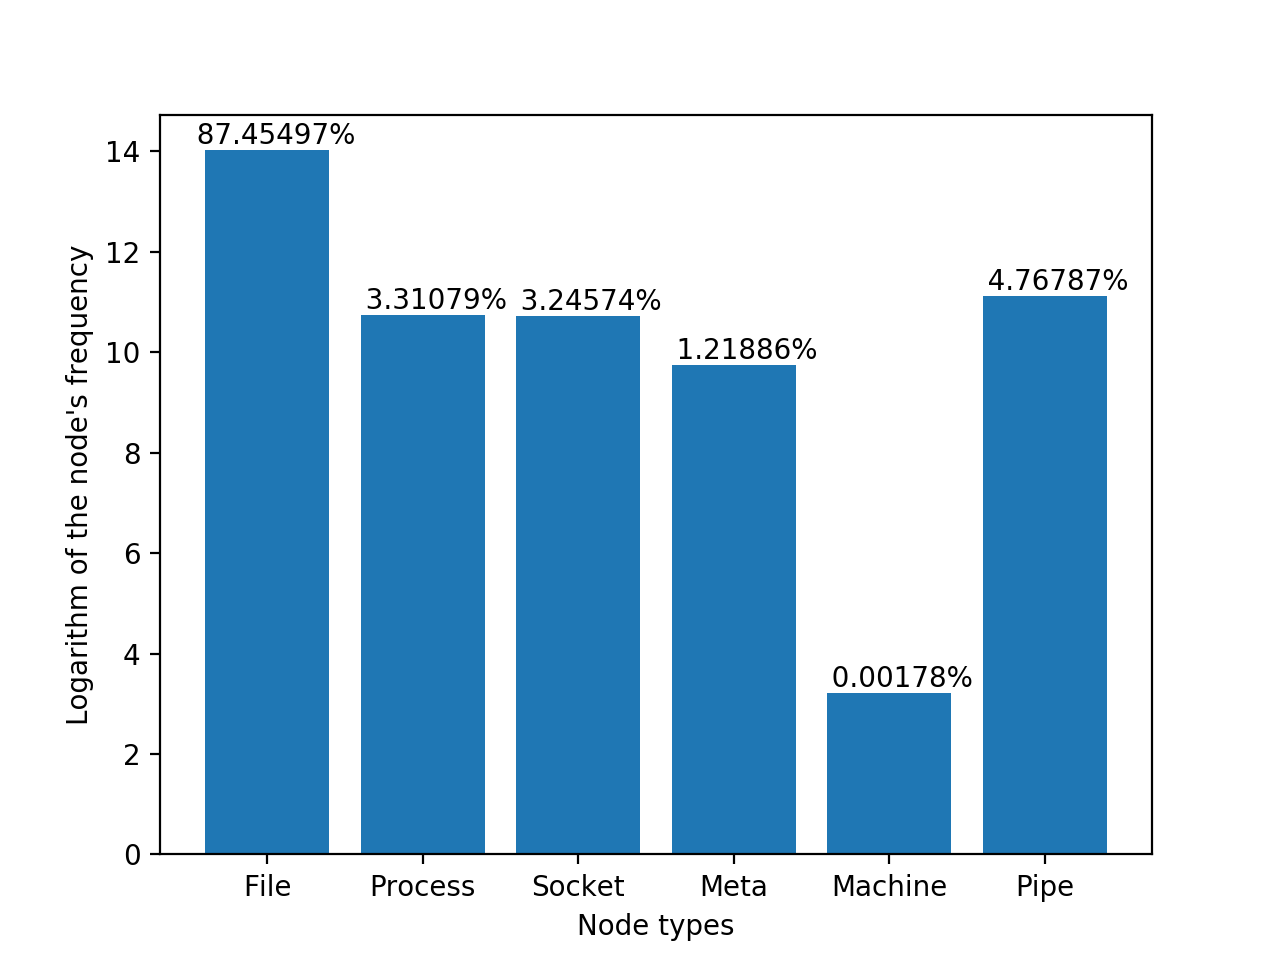
\includegraphics[width=0.7\textwidth]{graphics/node-freq-graph}
		\caption[\textbf{Log-scale node frequency}]{
			Bar chart above showing the log-scale node frequency in a database of $1,402,053$ nodes and $2,090,741$ edges. 
		}
	\end{figure}
	Relationships between nodes are illustrated by different types of edges. Some edges also illustrate how an object (File, Socket, etc.) evolves over time. This is done using the \textit{GLOB\_OBJ\_PREV} edge and helps us to easily visualize the different versions of an object.
	\begin{figure}[H]
		\centering
		\label{Figure 2.1.2}
		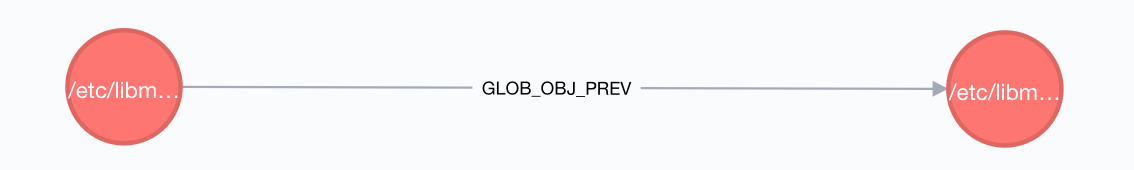
\includegraphics[width=0.7\textwidth]{graphics/GLOB_OBJ_PREV}
		\caption{
			Two versions of the same file connected via a GLOB\_OBJ\_PREV edge.
		}
	\end{figure}
	A number of the edge types also use a \textit{state} field, in order to provide further information regarding the relationship between two nodes. For example, in the case of a \textit{PROC\_OBJ} edge connecting a File to a Process, the \textit{state} field is used to show whether the Process reads/ writes to the File or if the File is the binary the Process is executed from. \textit{PROC\_OBJ} edges also connect Processes to Sockets. Here, the \textit{state} field can take values such as: \textit{Server} (if the Process uses the Socket to accept new connections), \textit{Client} (if the Process uses to Socket to connect to a different Process that acts as a server - which may or may not be on a different machine)  and \textit{RaW} (if the Process also reads and writes through the Socket).
	\begin{figure}[H]
		\centering
		\label{Figure 2.1.3}
		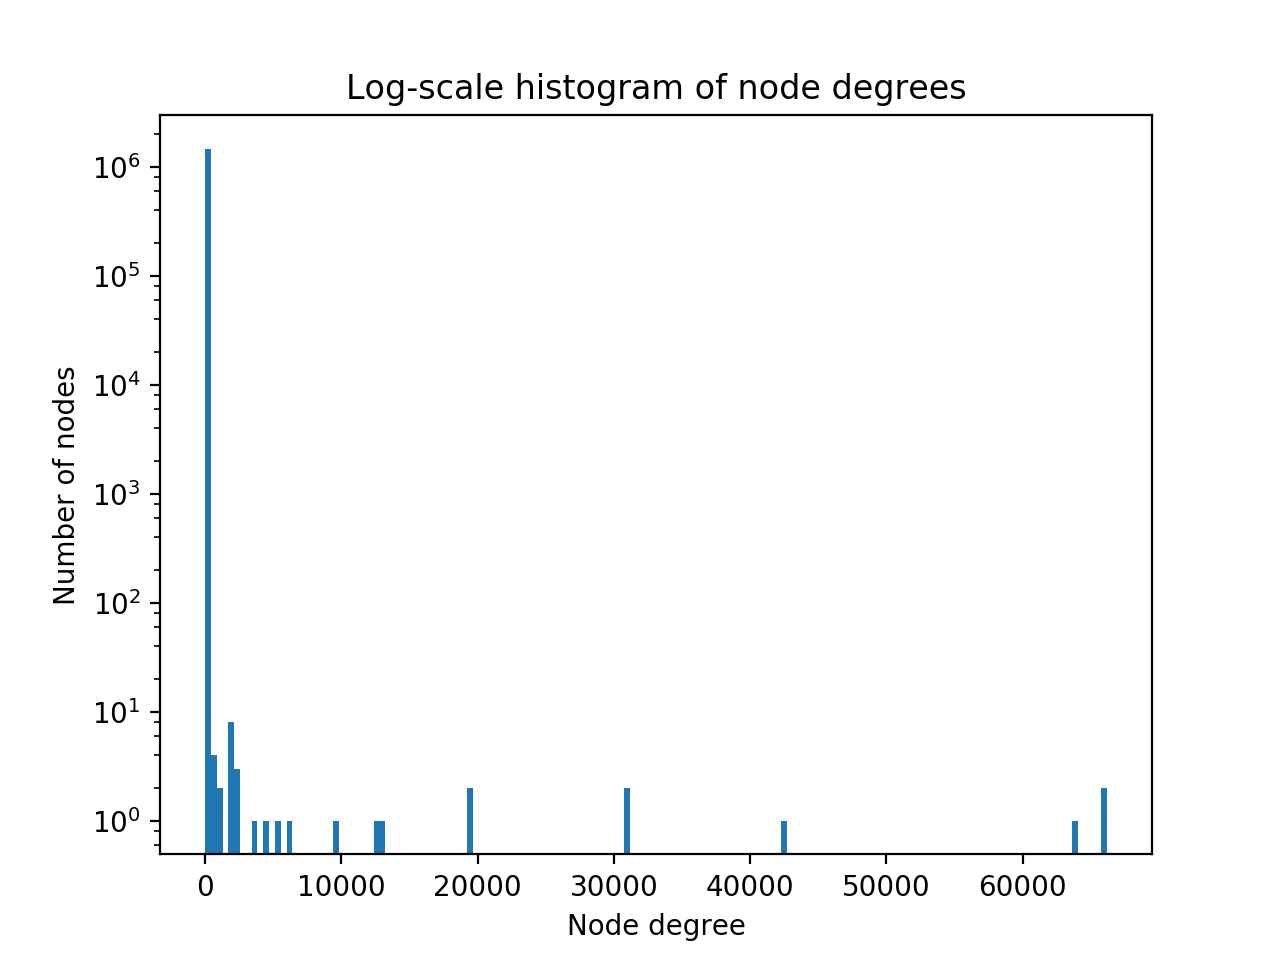
\includegraphics[width=0.7\textwidth]{graphics/node_degree_hist}
		\caption[Log-scale distribution of node degrees]{
			Log-scale histogram showing the distribution of node degrees, using the same graph as the one from Figure \ref{Figure 2.1.1} as source(i.e. $1,402,053$ nodes and $2,090,741$ edges).
		}
	\end{figure}
	 
	 The graphs resulting from tracing are very sparse, with a number of edges almost equal to the number of nodes. This observation is also sustained by the histogram in Figure \ref{Figure 2.1.3}, where we can observe that most of the nodes have degrees between 0 and 10, while there also are a few nodes with a very high degree (up to $60, 000$).
	 
	\subsection{Ground truths}
	In order to apply appropriate supervised learning algorithms, I had to build a labelled dataset of nodes from the raw data stored in graph format. This required setting a number of \textit{ground truths} of what a node of interest is. 
	\\ \\
	These ground truths are represented by a set of 6 rules, where I took into consideration a subset of node types: Files, Processes and Sockets. The rules are:
	\begin{enumerate}
		
		\item \textbf{Sockets that connect to an external IP: }Any socket that connects to an IP address other than 127.0.0.1 (localhost) can be considered a possible security breach because it could be used to leak information.
		
		\item \textbf{Files downloaded from the web and then executed: }Any file downloaded from the web can be suspicious, because we can not trust the source. Especially if it is executed, it can pose a real security threat to the system. The graph representation in the Neo4J database can be seen in Figure \ref{Figure 2.3}.
		\begin{figure}[H]
			\centering
			\includegraphics[width=0.7\textwidth]{graphics/downloaded-and-executed}
			\label{Figure 2.3}
			\caption{Graph representation of a file downloaded and then executed}
		\end{figure}
		In the figure above, Process1 writes the File while it is connected to the Socket and then Process2 starts, using File as binary.
		
		\item \textbf{File read from/ written to by a Processes that also opens a Socket to a different machine: }Here are two cases we need to treat separately. If the Process reads from the File, we face a potential leak of the File's contents. If the Process writes to the File, on the other hand, it might be the case that it corrupts its contents. This is a potential threat especially if the File is a sensitive file of the operating system (e.g. any file in /lib/ or /bin/). 
		
		\item \textbf{Processes that open a Socket to a different machine: }As mentioned at point 1, any Socket connecting to an external machine is a potential threat. In the same time, any process that opens a Socket to a different machine can be a source of suspicious behaviour, as well. 
		
		\item \textbf{Processes that runs suspicious commands: }Here, I define the term of \textit{suspicious command} as being one of the following bash commands:
		\begin{itemize}
			\item \textit{sudo} - gives the user running the Process root privilege. An attacker might use this to access OS-sensitive locations (such as /bin or /lib). 
			\item \textit{usermod/ groupmod} - an attacker might make use of these commands to change the running user's privileges and access files that it wouldn't otherwise have access to.
			\item \textit{chmod} - an attacker might use this command to change the access control to a specific File in order to make it accessible from external sources.
			\item \textit{rm -rf} - an ill-intended user might use this command to delete files crucial to the system. 
		\end{itemize}
	
		\item \textbf{Processes that writes to files in suspicious locations: }Here, I define the term of \textit{suspicious location} as being a location that is essential to the running of the system. These locations include:  \textit{/bin, /etc, /lib, /usr/bin, /usr/lib, /boot, /root, /dev, /etc/pwd}.
	\end{enumerate}
	\subsection{Data preprocessing}
	The implemented machine learning models only look at 3 of the 6 types of nodes: \textbf{File}, \textbf{Process} and \textbf{Socket} nodes. 
	\\ \\
	In order to achieve this, I had to define a set of features that would construct the \textit{feature vectors} representing each node. Furthermore, for graph-specific models (such as Graph Attention Networks, described in section \ref{Section 2.2.4})  I also built the adjacency matrix of the given graph. 
	\\ \\
	I defined 13 features that would describe each node, in the same time taking into account its 'neighbour'. For a Process, the neighbour is the closest File or Socket connected to it. Here, \textit{'the closest node'} is the node that with the closest timestamp to it. Similarly, for a File or Socket, the neighbour is the closest Process node connected to it.
		
	\begin{table}[!htbp]
		\centering
	\begin{tabular}{ |p{2.5cm}||p{3.2cm}|p{3.2cm}|p{2.7cm}|p{2.5cm}|}
		\hline
		\multirow{2}{3cm}{\textbf{Feature}} & \multicolumn{3}{|c|}{\textbf{Explanation}} & \multirow{2}{2cm}{Type}\\
		& Process & Socket & File &\\
		\hline
		\textit{Node type} & \multicolumn{3}{|c|}{The type of node used in this case (i.e. Process, Socket or File)} & \textbf{Categorical} \\
		\hline
		\textit{Neighbour type} & The closest node connected to it. Has to be one of File and Process & 
		\multicolumn{2}{|c|}{Will always be Process} & \textbf{Categorical}\\
		\hline
		\textit{Edge type} & \multicolumn{3}{|p{11cm}|}{The type of edge connecting the node to the neighbour. It will always be a $PROC\_OBJ$ edge, but the \textit{state} field can take multiple values, such as:  \textit{READ, WRITE, RaW, BIN, SERVER, CLIENT, NONE}.} & \textbf{Categorical}\\
		\hline
		\textit{Connected} & Whether the Process in question connects to a different machine via a Socket. & Whether the Sockets connects to an IP address other than 127.0.0.1 & Whether the File was downloaded from the web or not & \textbf{Binary} \\
		\hline
		\textit{Neighbour connected} & 
	\end{tabular}
	\end{table}


	\section{Machine learning models} \label{Section 2.2}
	
	\subsection{Baseline}	\label{Section 2.2.1}
	
	\subsection{Multi-perceptron model} \label{Section 2.2.2}
	
	\subsection{Convolutional Neural Network} \label{Section 2.2.3}
		
	\subsection{Graph Attention Network}	\label{Section 2.2.4}
		
	\subsection{Non-parametric techniques}	\label{Section 2.2.5}
	
	\section{API architecture} \label{Section 2.3}
	
	\section{Requirements analysis} \label{Section 2.4}
\end{document}